%% ============================================================================
%%  PES University — Capstone Project Report (Phase 2 and future phases)
%%  Template based on the UE23CS320B guidelines.
%%
%%  How to use:
%%    1. Fill in the \setup block below (project title, names, SRNs, etc.).
%%    2. Write your chapter content in chapters/*.tex.
%%    3. Drop figure images into figures/ and reference them from chapters.
%%    4. Compile with pdflatex (twice, so TOC/LOF/LOT and refs are correct).
%%       On Overleaf, the default recipe already does this.
%%
%%  Do NOT edit pesreport.cls unless you are changing the *visual* style.
%%  Content-only edits happen in this file and in chapters/*.tex.
%% ============================================================================

\documentclass{pesreport}

% ---- Optional extra packages -----------------------------------------------
% Uncomment what you need. `listings' is commonly wanted for code blocks.
% \usepackage{listings}
% \lstset{basicstyle=\footnotesize\ttfamily,breaklines=true,frame=single}

% ============================================================================
%   PROJECT METADATA — edit these values for your project
% ============================================================================

\projecttitle{An Intelligent Dental Assisting System for Dentists in Cavity and
Periodontal Disease Detection}
\projectid{PW26\_MHR\_06}
\coursecode{UE23CS320B}
\phasename{Capstone Project Phase - 2}
\phaseperiod{January - May 2026}
\phasesemester{sixth}
\reportperiod{Jan - May, 2026}          % appears in the page footer
\reporttitle{Capstone Project Phase - 2}% appears in the running header
\reportdept{Dept. of CSE}               % appears in the page footer

\guidename{Dr. Mamatha H R}
\guidedesignation{Designation, Department of CSE}
\chairperson{Dr. Shylaja S S}
\registrar{Dr. K S Sridhar}

% Team members — use \addteammember{Name}{SRN} for each author (up to ~6).
% The same list is reused on the title page, certificate, and declaration.
\addteammember{C S DEEPAK}{PES1UG23CS907}
\addteammember{CHENNUPATI GUNADEEP}{PES1UG23CS160}
\addteammember{ARCHANA}{PES1UG23CS098}
\addteammember{AVSN SAI SRUJAN}{PES1UG23CS123}

% Same team repeated for the declaration's SRN | Name | Signature table.
\addteamsign{C S DEEPAK}{PES1UG23CS907}
\addteamsign{CHENNUPATI GUNADEEP}{PES1UG23CS160}
\addteamsign{ARCHANA}{PES1UG23CS098}
\addteamsign{AVSN SAI SRUJAN}{PES1UG23CS123}

% ============================================================================
%   DOCUMENT BODY
% ============================================================================

\begin{document}

% ---- Front matter (no page numbers shown, no running headers/footers) ------
\pagestyle{pesfront}
\pagenumbering{roman}
\setcounter{page}{1}

\makepestitlepage
\makepescertificate
\makepesdeclaration

\begin{pesacknowledgement}
I would like to express my gratitude to \textbf{Prof. Guide Name}, Department
of Computer Science and Engineering, PES University, for his/her continuous
guidance, assistance, and encouragement throughout the development of this
UE23CS320B -- Capstone Project Phase -- 2.

I am grateful to the project coordinator, \textbf{Prof. Gayathri R S}, for
organising, managing, and helping with the entire process.

I take this opportunity to thank \textbf{Dr. Shylaja S S}, Chairperson,
Department of Computer Science and Engineering, PES University, for all the
knowledge and support I have received from the department. I would like to
thank \textbf{Dr. K S Sridhar}, Registrar, PES University, for his help.

I am deeply grateful to \textbf{Prof. Jawahar Doreswamy}, Chancellor, PES
University, and \textbf{Dr.\ Surya\-prasad~J}, Vice-Chancellor, PES University,
for providing various opportunities and enlightenment every step of the way.
Finally, this project could not have been completed without the continual
support and encouragement received from my family and friends.
\end{pesacknowledgement}



\begin{abstract}

Accurate interpretation of dental panoramic radiographs(OPGs) is a complex and challenging task due to the subtle nature of early carious lesions and periodontal bone less, especially for early-stage dental practitioners. Manual analysis is very time consuming, subjective, and results are prone to vary between different examiners. Existing deep learning approaches in this domain are primarily focused on single tasks and are narrowly scoped, addressing either caries detection or periodontal assessment alone, lacking clinical explainability and severity grading.


This project presents an unified, end-to-end, multi-task deep learning pipeline that analyzes the dental radiographs to detect caries with severity grading and assess periodontal disease via alveolar bone loss estimation . In this approach, the system decomposes each OPG into individual tooth regions using YOLO-based detection with FDI numbering, which enables localized analysis and improved interpretability,then ResNet18 classifier is applied for binary caries detection and severity grading, which classifies them into Caries vs. Deep Caries. Periodontal bone loss is assessed using pathology mask overlap on expanded tooth crops that are derived from the dental dataset. Explainability is incorporated via Grad-CAM visualizations to support clinical decision making. The system outputs a structured, tooth-level diagnostic report aligned with the FDI standards, designed to assist junior clinicians and dental students in consistent, interpretable radiographic assessment.
\end{abstract}

% ---- Table of Contents, List of Figures, List of Tables -------------------
\tableofcontents
\clearpage

\listoffigures
\clearpage

\listoftables
\clearpage

% ---- Main matter: switch to Arabic page numbers and running header/footer --
\startcontentpages

%% Chapter 1 - Introduction

\chapter{Introduction}
\label{ch:introduction}

Dental panoramic radiography, also referred to as Orthopantomography (OPG),
provides a single two-dimensional view of the full dentition, alveolar bone,
maxilla, mandible, and surrounding anatomical structures. Because one image
captures most of the clinically relevant oral region, OPGs are routinely used
for screening dental caries, periodontal bone loss, impacted teeth, and other
oral pathologies. Their practical value is high, but so is the difficulty of
interpretation: weak local contrast, overlapping structures, projection
distortion, and subtle early lesions all increase the risk of missed or
inconsistent findings.

The present project aims to build an intelligent dental assisting system that
uses deep learning to move from a full OPG to a structured tooth-wise report.
The target system is tooth-centric. Instead of classifying the full radiograph
as a single unit, the OPG is first decomposed into tooth-level regions and each
tooth is then analyzed through task-specific models. This design is clinically
motivated: dentists reason per tooth, and an assistive system is only useful if
it can localize its findings and map them to a standard numbering scheme.

The broader survey work conducted alongside this project also reinforced a
system-level conclusion that directly shaped Phase 2: current dental AI
literature is strong on isolated subtasks, but weak on complete OPG-to-report
workflows. This is why the present report emphasizes modular implementation and
honest integration status instead of claiming a fully finished clinical system.

At the project level, the intended end-to-end workflow is: full OPG input,
tooth detection, FDI numbering, caries analysis on tight tooth crops,
periodontal analysis on expanded bone-aware tooth crops, and final report
generation. However, this report is restricted to work completed up to the
current Phase 2 milestone. The major completed contributions are the
dataset-engineering and model-development steps for the caries and periodontal
branches. On the caries side, a collaborator has built a two-stage ResNet18
cascade on DENTEX tooth crops. On the periodontal side, the work completed in
this repository includes Tufts annotation exploration, correction of critical
data parsing bugs, tooth-level crop generation, overlap-based label assignment,
binary bone-loss classification, overlap-based severity classification, and an
exploratory CEJ-based estimation module.

One of the most important outcomes of this phase is that the periodontal branch
is already supported by reproducible code and measured results. The bone-loss
binary classifier trained on resampled Tufts crops achieved a validation
macro-F1 of 0.9233, while the overlap-based severity model achieved a macro-F1
of 0.7208. The CEJ-based heuristic branch was investigated because it is closer
to the clinical standard, but the current OPG-based formulation remains
insufficiently reliable and is therefore treated as future work rather than the
primary reporting pathway.

This report is organized as follows. Chapter~\ref{ch:architecture} describes
the target system architecture and clarifies which parts are already
implemented. Chapter~\ref{ch:methodology} documents the datasets, preprocessing
choices, model configurations, and training design used so far.
Chapter~\ref{ch:implementation} presents the implemented modules in the current
repository and notebooks. Chapter~\ref{ch:results} summarizes the quantitative
and qualitative findings supported by the saved artifacts. Finally,
Chapter~\ref{ch:conclusion} concludes the report and outlines the most
immediate next steps toward full pipeline integration.

%% Chapter 2 — Literature Survey
%% Guideline target: ~2 pages.
%%
%% Keep this tight. In Phase 2 the literature survey is NOT the main deliverable
%% — reviewers have already seen your Phase 1 survey. Summarise only what is
%% directly relevant to the architecture and methodology you actually built.
%%
%% Style convention for this template: one subsection per paper, each ending
%% with a one-line "Relevance to our work" sentence.

\chapter{Literature Survey}
\label{ch:literature}

% ---------------------------------------------------------------------------
\section{Paper Title Goes Here}
\label{sec:lit-paperA}

\textbf{Authors:} Author et al. \quad \textbf{Year:} 20XX \quad
\textbf{Venue:} Journal / Conference

\textit{[Replace.] One paragraph summarising what this paper does, the
dataset used, and the headline result. Do not copy from the paper — paraphrase.}

\textit{[Replace.] One paragraph on limitations of the paper and how your
project addresses or extends them.}

% Example of an in-line figure reference (image must exist under figures/):
% \begin{figure}[htbp]
%   \centering
%   \includegraphics[width=0.8\linewidth]{figures/lit_paperA_arch.png}
%   \caption{Architecture proposed by Author et al.}
%   \label{fig:lit-paperA-arch}
% \end{figure}

% ---------------------------------------------------------------------------
\section{Second Paper Title}
\label{sec:lit-paperB}

\textit{[Replace with content, structured like the section above.]}

% ---------------------------------------------------------------------------
\section{Research Gaps}
\label{sec:lit-gaps}

\textit{[Replace.] Summarise the gaps identified across the surveyed work
that motivate your project's contribution. Bullet points are acceptable here.}

\begin{itemize}
  \item \textit{[Gap 1]}
  \item \textit{[Gap 2]}
  \item \textit{[Gap 3]}
\end{itemize}

%% Chapter 3 — Architecture with Explanation
%% Guideline target: 1–2 pages.
%%
%% This chapter should present the end-to-end system architecture — the
%% highest-level picture of what flows into what. One architecture diagram
%% is expected. Do NOT put implementation details here; that is Chapter 5.

\chapter{Architecture with Explanation}
\label{ch:architecture}

\section{System Overview}
\label{sec:arch-overview}

The proposed system follows a pipeline-based tooth-centric architecture that mimics the clinical diagnostic workflow. This process is broken down into multiple stages each responsible for a particular task. Instead of processing a single image for classification , the system decomposes it into individual tooth regions. The end-to-end pipeline consists of the following sequential stages: OPG input, image enhancement and normalization, tooth detection and FDI numbering, multi-disease detection, explainable AI, and structured report generation.

% Architecture figure — replace the placeholder with your diagram image.
\begin{figure}[htbp]
  \centering
   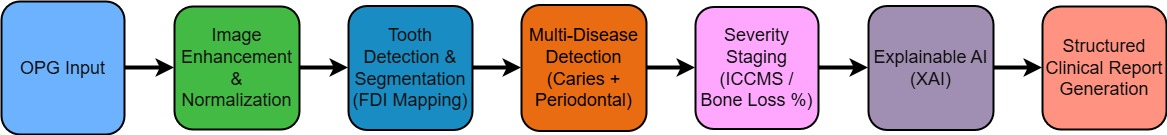
\includegraphics[width=0.9\linewidth]{fig1.jpeg}
  
  \caption{End-to-end system architecture.}
  \label{fig:architecture}
\end{figure}

\section{Component Description}
\label{sec:arch-components}


\subsection{OPG Input}
The first stage takes a panoramic radiograph as input. OPG images provide a complete view of the dentition and the surrounding structures, making them very useful for detecting multiple conditions. However, these images are often affected by low contrast, noise, and overlapping anatomical structures , which can make interpretation difficult. Due to these challenges, the raw image cannot be used directly for accurate analysis and requires preprocessing.

\subsection{Image Enhancement and Normalization}
The  image enhancement and normalization stage is required for improving the quality and consistency of the input data. Techniques such as contrast enhancement and intensity normalization are applied to bring out the subtle features that may help in detecting early-stage caries or slight variations in bone levels. Further, all images are resized and standardized to ensure compatibility with the deep learning models used in later stages. This step plays an important role in reducing variability across datasets and significantly improving the model’s performance .


\subsection{Tooth Detection and Segmentation}
Following the preprocessing, the system performs tooth detection and segmentation. A pretrained YOLO model trained on the dataset is used to process the full OPG image. It produces bounding box detections for each visible tooth. Then, these detections are mapped to standard FDI numbers (11-    48), allowing each tooth to be identified uniquely. These transformations allow to reduce noise by isolating each tooth, which helps in interpreting accurate results. This step is necessary for generating a clinically useful structured report at the later stage.



\subsection{Multi-Disease Detection}
In this stage the system performs multi-disease detection to identify both dental caries and periodontal disease detection within the same framework. For each tooth detected, two image crops are extracted, tightly cropped regions around the crown is passed to caries classification model and the larger expanded crop surrounding the alveolar bone region is passed to periodontal assessment model. This separation of analysis pathways improves accuracy and 
allows caries and bone loss to be evaluated from the same tooth bounding box .

\subsection{Severity Staging}
After detecting the presence of disease, the system performs severity staging to provide more clinically useful interpretations. For dental caries, severity is estimated based on the progression levels. For periodontal disease, bone loss percentage is calculated, which provides a quantitative measure of the disease progression. This stage is very critical as the detection alone is not enough for clinical decision making. BY including the severity grading, the system supports treatment planning.


\subsection{Explainable AI }
The system incorporates Grad-CAM explainability for providing visual explanations, which highlights the regions of the image that contributed to the model's prediction. These visual explanations allows clinicians to verify the reasoning behind the system's output are based on relevant features, enhancing transparency and trust.

\subsection{Structured Clinical Report Generation}
The final stage involves generating a structured clinical report. All predictions, including tooth-wise disease detection, severity classification, FDI tooth ID, and the corresponding Grad-CAM visualizations, are integrated into a final output. Instead of providing isolated predictions, the system provides a comprehensive summary that closely resembles a real diagnostic report.



\section{Design Rationale}
\label{sec:arch-rationale}

The tooth-centric decomposition approach was selected over other approaches like image-level classification, such as that used  by Bhoopalan et al. (2026), which achieved 96\% OPG-level accuracy using Vision Transformers (ViT). While effective at a global level, such approaches do not provide the per-tooth localization required for detailed clinical reporting. By focusing on individual teeth rather than the entire image,  the system improves interpretability and allows more precise predictions.

End-to-end transformer-based models were also taken into consideration but not adopted at this stage due to their high annotation requirements. Currently, there is no large-scale, multi-disease, multi-center public dataset of dental panoramic radiographs (OPGs) that supports such training. Additionally, their inference latency is approximately 40 seconds per image which makes them impractical for real-time clinical applications.

In contrast, a pipeline-based convolutional neural network (CNN) approach offers improved interpretability, modularity, and computational efficiency. Each component in the pipeline can be trained independently and updated as improved datasets or architectures become available. Explanability is also an important part of this design. Rather than treating the model as a black box, the system provides visual justifications for its predictions, making it more transparent and clinically more trustable.


%% Chapter 4 — Methodology
%% Guideline target: 1–2 pages.
%%
%% Methodology describes the *approach*, not the *code*. Datasets, splits,
%% preprocessing choices, model selection criteria, training strategy,
%% evaluation metrics. A reader should be able to replicate the EXPERIMENTAL
%% DESIGN (not the implementation) from this chapter alone.

\chapter{Methodology}
\label{ch:methodology}

\section{Dataset}
\label{sec:method-dataset}

Three datasets were used in this project, each one of them is selected based on the type of annotations relevant to corresponding module in the pipeline.

The DENTEX dataset (Dental Enumeration and Diagnosis on Panoramic X-rays) consists of 
1,005 panoramic radiographs sourced from multiple institutions. It provides bounding box 
labels for teeth as well as labels for dental caries. These annotations are used for training the tooth detection model (YOLO) and the caries classification model (ResNet18). The dataset includes two main pathology classes, namely Caries and Deep Caries, which also support severity-based 
classification.

The Tufts Dental Database is primarily used for periodontal bone loss analysis. It contains around 1,000 panoramic radiographs along with multiple annotation types, including expert text labels, bounding boxes, and pathology masks. During data exploration, it was observed that only a subset of the data contains all required annotations simultaneously. After filtering, 423 images were selected as the working dataset for the bone loss pipeline.These images were further processed to generate tooth-level crops, resulting in a total of 22,806 samples. However, a major challenge observed in this dataset is severe class imbalance. 
Approximately 96\% of the samples correspond to normal teeth, while only 4\% represent diseased cases. This imbalance occurs because each image contains many teeth, and even in images with disease, most teeth are still healthy. As a result, standard training methods such as cross-entropy loss tend to perform poorly, requiring additional handling strategies such as resampling.


The CariesXrays dataset contains 6,000 high-quality panoramic radiographs with over 13,000 expert-annotated caries bounding boxes. This dataset is intended to improve the robustness of the caries detection module, particularly in challenging cases such as teeth with metallic restorations. Integration of this dataset is planned for future work.
Overall, the use of multiple datasets is necessary due to the lack of a single dataset containing all required annotations. However, this introduces challenges such as annotation inconsistency and class imbalance, which are addressed through preprocessing and data selection techniques.




\begin{table}[htbp]
  \centering
  \caption{Dataset summary.}
  \label{tab:dataset-summary}
  \begin{tabular}{@{}llll@{}}
    \toprule
    Split & Images & Positive class \% & Notes \\
    \midrule
    Train & -- & -- & -- \\
    Val   & -- & -- & -- \\
    Test  & -- & -- & -- \\
    \bottomrule
  \end{tabular}
\end{table}

\section{Preprocessing}
\label{sec:method-preprocessing}

\subsection{Bounding Box Correction}
During the dataset construction it has been observed that the raw bounding box coordinates in the Tufts dataset were not in the standard format [x,y,w,h]. Without the correction, all crop extractions would have been geometrically incorrect. The correction applied is: 
x = x1, y = y1 , w = x2 - x1 , h = y2 - y1 ,
with the x and y axes swapped. After conversion, tooth bounding box dimensions were verified to be anatomically plausible, with width ranging from a minimum to a maximum across the 26,005 annotated teeth.

\subsection{Asymmetric Expanded Crop for Bone Loss Assessment}
Tooth crops for periodontal assessment are expanded asymmetrically: 1.5× in the horizontal direction and 2.0× in the vertical direction. This asymmetric design reflects the anatomical reality that teeth have a mean aspect ratio of approximately 0.35 (they are three times taller than wide). Symmetric expansion would cause excessive horizontal bleed into adjacent teeth, while insufficient vertical expansion would fail to capture the alveolar bone below the root apex, which is the key region for bone loss assessment. The expansion formula computes the centre of the original bounding box, then extends outward by the scaled half-widths and half-heights, clipping to image boundaries.

\subsection{Overlap-Metric based Label}
The standard Intersection over Union metric was explicitly rejected for labelling bone loss crops. The expert pathology masks in the Tufts dataset are sparse: lesion annotations occupy only 0.5–2\% of the total crop area. When IoU is applied to these sparse annotations, even true positive cases produce IoU values near zero, because the union term is dominated by the large crop area. The overlap metric used instead is: overlap = (non-zero mask pixels inside the expanded crop) / (total crop area). A threshold of 0.01 (1\% coverage) was adopted as the label boundary after visual inspection of the overlap distribution, distinguishing genuine periapical pathology from noise-level mask fragments.


\subsection{Bounding Box Jitter for YOLO Noise Simulation}
To prevent distribution mismatch at inference, a random perturbation of ±15\% is applied to the bounding box coordinates during dataset construction. This simulates the noise introduced by YOLO detection at inference time. Without this jitter, the model trains on geometrically perfect ground-truth crops but receives slightly misaligned crops at inference, causing a systematic performance drop. Random offsets dx, dy, dw, and dh are sampled uniformly and applied to the box, with clipping to ensure the jittered box remains within image boundaries and retains minimum dimensions.

\subsection{CLAHE Preprocessing for CEJ Estimation}
The CEJ estimation module applies Contrast Limited Adaptive Histogram Equalization (CLAHE) with a clip limit of 2.0 and an 8×8 tile grid before landmark detection. OPG crops exhibit significant local contrast variation due to acquisition geometry, and CLAHE normalizes this variation to make bone-to-tooth boundaries more visible. A gentle Gaussian blur (sigma = 1.5) is applied after CLAHE to suppress pixel noise without destroying structural edges. This preprocessing step was a key improvement in version 2 of the CEJ pipeline, contributing to the increase in successful CEJ detection rate compared to the raw-grayscale version 1 baseline.

\subsection{Data Augmentation}
The severity classification dataset is constructed from positive crops (bone loss class 1) from the binary dataset. Because the Severe class (overlap > 0.15) is substantially underrepresented relative to the Mild class (overlap 0.01–0.05), augmentation copies are generated for minority classes during dataset construction using random horizontal flip, random rotation within 12 degrees, colour jitter with brightness factor 0.25 and contrast factor 0.15, and random translation within 6\% in both axes. All augmented copies from the same source image are kept in the same split to prevent data leakage.


\subsection{Handling Class Imbalance }
To address the class imbalance, a corrected resampled dataset is constructed from the raw processed dataset output before binary model training. The resampling strategy has two components. First, normal crops are undersampled from 17,473 training samples down to approximately 2,500 using a stratified approach: each source image contributes a proportional share of the 2,500 target, ensuring that no single image dominates the normal class after undersampling. Second, the 739 original diseased training crops are kept in full, and two augmented copies are generated for each using random horizontal flip, random rotation within 10 degrees, colour jitter with brightness 0.2 and contrast 0.1, and random affine translation within 5\%, bringing the total diseased training crop count to approximately 2,217. The resulting train set ratio of approximately 1.1× is close to balanced. Critically, the validation set is kept entirely untouched — no resampling is applied to val — so that evaluation metrics reflect the real-world class distribution rather than a corrected one.



\section{Model Architecture}
\label{sec:method-model}

All classification modules use ResNet18 with ImageNet pre-training and the final fully connected layer replaced to match the number of output classes. For caries severity classification (No Caries / Caries / Deep Caries), the output layer maps 512 features to 3 classes. For bone loss binary detection, the output layer maps to 2 classes. For the three-class bone loss severity model (Mild / Moderate / Severe), the same ResNet18 backbone maps to 3 classes. ResNet18 was selected over larger variants after finding that ResNet50 trained on the same dataset exhibited a training-validation accuracy gap of 14 percentage points compared to 7 for ResNet18, indicating insufficient data to support the larger model capacity. The tooth detection module uses a pre-trained YOLOv8 model fine-tuned on DENTEX dataset.

\section{Training Strategy}
\label{sec:method-training}

\textit{[Replace.] Optimiser, loss function, learning-rate schedule, batch
size, early-stopping criterion, class-weighting if any. Include the exact
epoch count and hardware used.}

\section{Evaluation Metrics}
\label{sec:method-metrics}

All classification modules are evaluated using per-class Precision, Recall, and F1-score, plus macro-averaged F1. Raw accuracy is not used as the primary metric given class imbalance. For the bone loss binary module, Recall for the positive class (bone loss present) is prioritized, because in a screening context false negatives are clinically more harmful than false positives. For the severity modules, macro-F1 is the selection metric, ensuring no class is ignored during model selection. Image-level stratified train-validation splits are used for all modules, with all crops from the same OPG kept within the same split to prevent data leakage from jittered augmentation copies. A leakage check is performed after every split by verifying that the intersection of training and validation image stems is empty.

% Example equation — uses chapter.section numbering automatically.
\begin{equation}
  \label{eq:f1}
  F_1 = \frac{2 \cdot \mathrm{Precision} \cdot \mathrm{Recall}}{\mathrm{Precision} + \mathrm{Recall}}
\end{equation}

%% Chapter 5 — Implementation (Salient Modules)
%% Guideline target: ~2 pages.
%%
%% This is where the actual code-level details go. Module-by-module walkthrough.
%% Include representative code snippets (use `listings` if you want syntax
%% highlighting; it is already available on Overleaf). Keep snippets short —
%% no one wants to read a whole file in a report.

\chapter{Implementation}
\label{ch:implementation}

\section{Technology Stack}
\label{sec:impl-stack}

The system is implemented in Python 3.10. The deep learning framework is PyTorch 2.0 with torchvision 0.15. Tooth detection uses Ultralytics YOLOv8. Dataset loading and annotation parsing use custom parsers for the Tufts JSON format and DENTEX COCO-format annotations. Image processing uses OpenCV 4.8 and PIL/Pillow 10.0. Signal processing for the CEJ estimation module uses scipy.signal (Savitzky-Golay filtering) and scipy.ndimage (Gaussian filtering). Model evaluation uses scikit-learn for F1, classification reports, and confusion matrices. Development and training were conducted on Google Colab using T4 and A100 GPU instances. 


\section{Module 1: \textit{Caries Cascade Classifier }}
\label{sec:impl-module1}



\section{Module 2: \textit{Dataset Exploration and Annotation Parsing }}
\label{sec:impl-module2}


\section{Module 3: \textit{Bone Loss Dataset Construction}}
\label{sec:impl-module3}

\section{Module 4: \textit{Bone Loss Binary Classifier Training }}
\label{sec:impl-module4}

\section{Module 5: \textit{Bone Loss Severity Classification}}
\label{sec:impl-module5}

\section{Module 6: \textit{CEJ- based Bone Loss Estimation}}
\label{sec:impl-module6}




\section{Integration and Pipeline Orchestration}
\label{sec:impl-integration}

The pipeline is orchestrated by a central controller script that accepts an OPG image path and returns a JSON report. The execution sequence is: (1) YOLOv8 tooth detection and FDI numbering; (2) per-tooth dual-path processing where the tight crop is passed to the ResNet18 caries classifier and the expanded crop is passed to the bone loss binary classifier; (3) for teeth flagged as bone-loss positive, the expanded crop is additionally passed to the severity classifier; (4) for all teeth with non-normal caries predictions, Grad-CAM is computed on the last convolutional layer of the ResNet18 caries model; (5) the filtering stage removes teeth where both modules report normal findings; (6) the report generator serializes filtered tooth records to JSON and produces a PDF containing the annotated OPG, per-tooth findings table, and Grad-CAM thumbnails. The pipeline is modular: each module can be upgraded independently without modifying the orchestration layer.

%% Chapter 6 - Results

\chapter{Results}
\label{ch:results}

\section{Quantitative Results}
\label{sec:results-quant}

The strongest quantitative result obtained in the current phase is the binary
bone-loss classifier, which achieved a validation macro-F1 of 0.9233 on the
held-out Tufts validation split. The overlap-based severity classifier and the
caries severity stage are weaker but still useful intermediate baselines,
whereas the CEJ branch remains exploratory.

\begin{table}[htbp]
  \centering
  \caption{Validated results currently supported by saved artifacts.}
  \label{tab:results-comparison}
  \begin{tabular}{@{}lcccc@{}}
    \toprule
    Module & Accuracy & Key class recall & Specific note & Macro-F1 \\
    \midrule
    Bone-loss binary & -- & 0.8305 & Specificity = 0.9953 & 0.9233 \\
    Bone-loss severity & -- & -- & Mild F1 = 0.80 & 0.7208 \\
    Caries severity (initial phase 2) & 0.80 & Deep-caries recall = 0.59 & Preserved notebook output & 0.73 \\
    Caries severity (best preserved phase 2) & 0.81 & Deep-caries recall = 0.84 & Final refined run & 0.77 \\
    \bottomrule
  \end{tabular}
\end{table}

The quantitative evidence for the caries branch requires one clarification. The
exported collaborator notebook preserves the validation reports for the second
stage of the cascade (caries versus deep caries), but the final printed report
for the first-stage caries versus no-caries classifier is not present in the
checked notebook artifact. Therefore, Table~\ref{tab:results-comparison}
reports only the validated caries-stage outputs that can be directly recovered
from the repository.

\begin{figure}[!htbp]
  \centering
  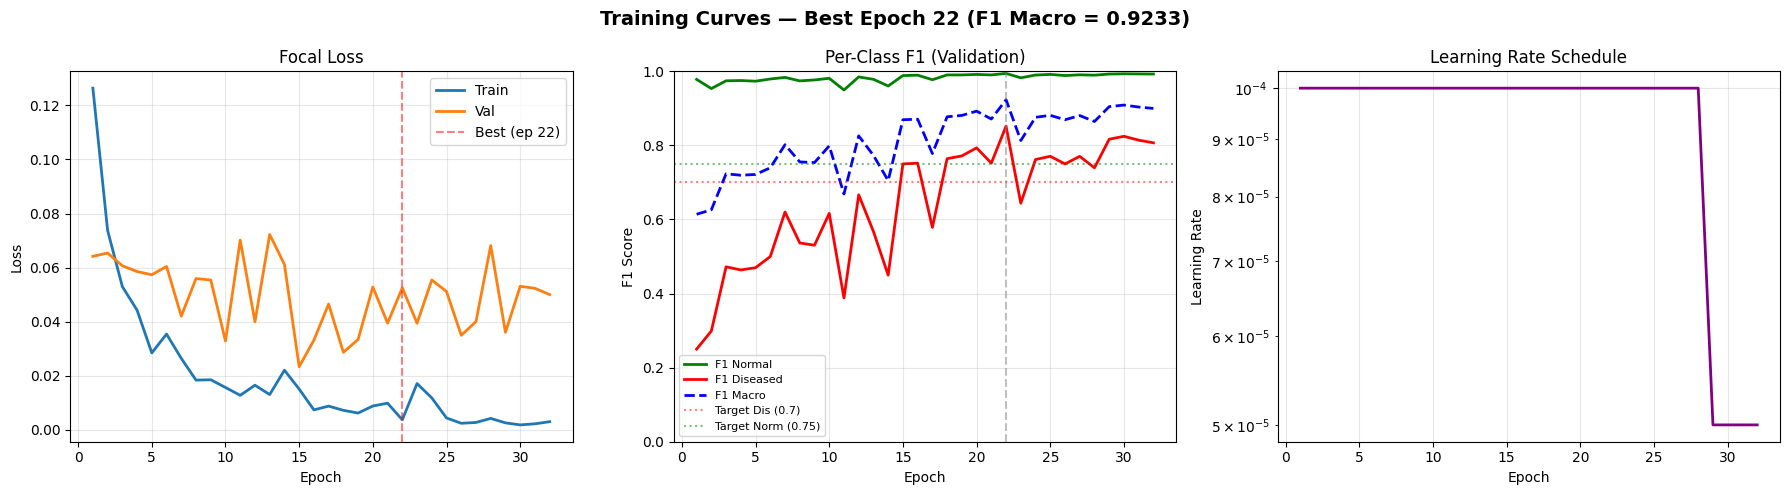
\includegraphics[width=0.82\linewidth]{figures/bone_loss_training_curves.png}
  \caption{Training and validation curves for the binary bone-loss classifier.}
  \label{fig:bone-loss-training-curves}
\end{figure}

Figure~\ref{fig:bone-loss-training-curves} shows stable optimization behavior
for the binary periodontal model. The best checkpoint was selected from the
validation trajectory, not simply from the final epoch.

\begin{table}[htbp]
  \centering
  \caption{Detailed periodontal branch results.}
  \label{tab:periodontal-results}
  \begin{tabular}{@{}lccc@{}}
    \toprule
    Metric & Binary bone loss & Severity classifier & CEJ v2 \\
    \midrule
    Validation set size & 1,558 & positive subset & 296 crops \\
    Sensitivity / recall & 0.8305 & -- & reliable on 62.5\% \\
    Specificity & 0.9953 & -- & -- \\
    Macro-F1 & 0.9233 & 0.7208 & -- \\
    Exact agreement with overlap labels & -- & -- & 15.1\% \\
    Agreement within \(\pm 1\) class & -- & -- & 61.6\% \\
    \bottomrule
  \end{tabular}
\end{table}

\begin{figure}[!htbp]
  \centering
  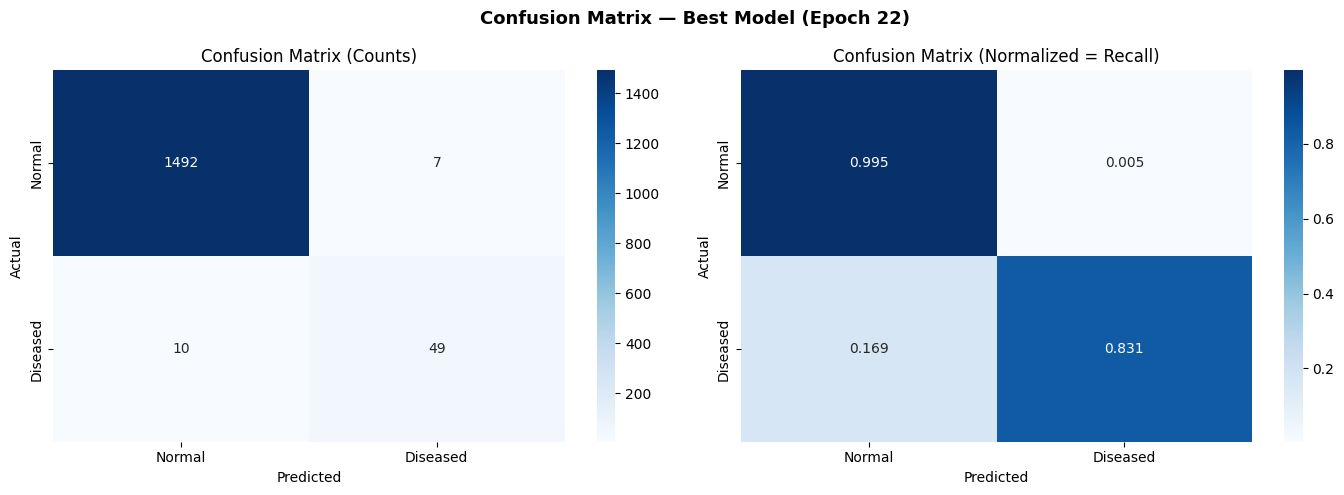
\includegraphics[width=0.58\linewidth]{figures/bone_loss_confusion_matrix.png}
  \caption{Confusion matrix of the binary bone-loss classifier on the validation split.}
  \label{fig:bone-loss-cm}
\end{figure}

Figure~\ref{fig:bone-loss-cm} highlights the strongest property of the binary
model: very low false-positive rate with still useful diseased-case recall.

\section{Qualitative Results}
\label{sec:results-qual}

Two qualitative observations are consistent across the experiments. First, the
binary periodontal classifier is robust on clearly normal and clearly diseased
crops, which suggests that the asymmetric crop design successfully exposes the
relevant bone context to the network. Second, the failure cases cluster around
more ambiguous boundaries: mild versus moderate bone loss, and caries versus
deep caries. This is expected because both tasks depend on relatively small
visual differences within a limited dataset.

The CEJ branch provides the clearest failure analysis. It can usually locate a
candidate landmark pattern after CLAHE preprocessing, but overlapping
structures, metallic restorations, and anterior-tooth morphology variations
often make the measurement clinically unreliable. This is precisely why the CEJ
branch is not used as the primary severity output despite being conceptually
closer to the periodontal gold standard.

\begin{figure}[!htbp]
  \centering
  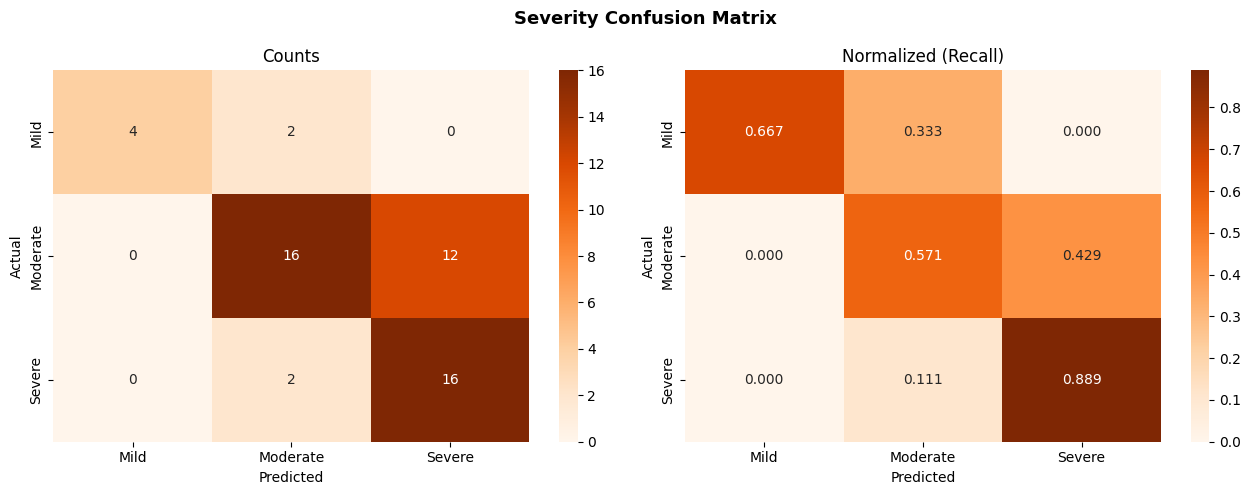
\includegraphics[width=0.58\linewidth]{figures/bone_loss_severity_confusion_matrix.png}
  \caption{Confusion matrix for the overlap-based three-class bone-loss severity model.}
  \label{fig:bone-loss-severity-cm}
\end{figure}

Figure~\ref{fig:bone-loss-severity-cm} shows that severity staging is harder
than binary detection. Most errors occur between adjacent severity categories,
which is clinically more plausible than random confusion.

% Suggested figures for the final camera-ready version:
% 1. Bone-loss crop with expert mask overlay and predicted class.
% 2. CEJ v2 success case with detected landmarks and confidence score.
% 3. CEJ v2 failure case showing why the heuristic is unreliable on some OPGs.
% 4. Caries severity examples: caries vs deep-caries confusion pair.

\section{Ablation / Comparative Analysis}
\label{sec:results-ablation}

Although a formal ablation table is not yet available for every branch, three
comparative findings are already supported by the current artifacts.
\begin{enumerate}
  \item Correct annotation parsing mattered more than model complexity.
  Fixing the Tufts \texttt{External ID} join bug and the bounding-box coordinate bug
  was essential; without these fixes, the periodontal pipeline would have been
  trained on mismatched labels and incorrect crops.
  \item Overlap-based severity is currently more practical than CEJ-based
  severity on panoramic OPGs. The CEJ branch is clinically attractive, but its
  agreement with overlap-derived labels remains too weak to use as the primary
  severity estimator.
  \item The caries cascade benefited from low-learning-rate refinement in
  phase 2. The preserved results improved from macro-F1 0.72 to 0.77 and
  deep-caries recall from 0.78 to 0.84 after reweighting and additional
  fine-tuning.
\end{enumerate}

\begin{figure}[!htbp]
  \centering
  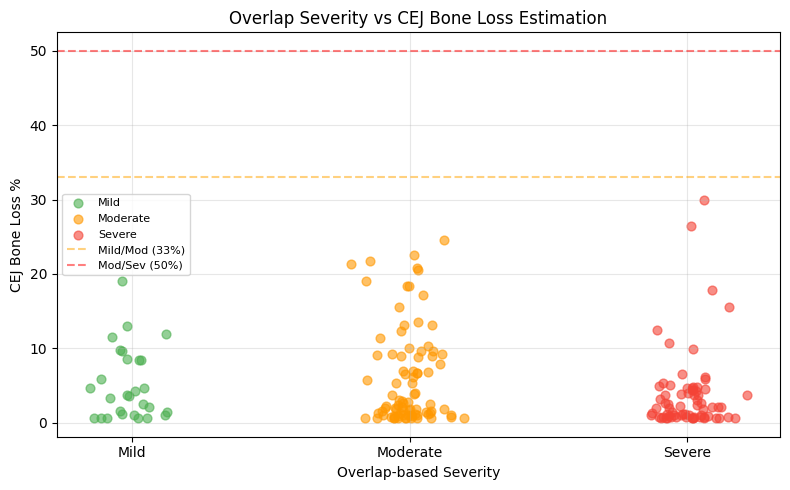
\includegraphics[width=0.62\linewidth]{figures/cej_agreement_analysis.png}
  \caption{Agreement analysis between CEJ-based estimation and overlap-based severity labels.}
  \label{fig:cej-agreement}
\end{figure}

Figure~\ref{fig:cej-agreement} supports the decision to retain CEJ as an
exploratory branch. The current agreement is informative, but not strong enough
for primary severity reporting on panoramic OPGs.

\section{Discussion}
\label{sec:results-discussion}

The main result of this phase is that the periodontal branch is not merely an
idea but an implemented and quantitatively validated subsystem. A standard
ResNet18, when paired with correct tooth-level crop construction and imbalance
handling, is already strong enough to detect bone loss reliably on the held-out
Tufts validation set. This is the clearest technical success in the repository.

The limitations are equally important. The overall project is still modular
rather than integrated; there is no full-OPG inference script yet. The caries
branch depends on notebook artifacts with incomplete experiment logging for the
first-stage metrics. The CEJ branch remains exploratory, and no calibrated
confidence layer or Grad-CAM reporting layer has been integrated into the final
workflow. These gaps define the next phase of work rather than weakening the
value of the completed modules.

%% Chapter 7 — Conclusion and Future Work
%% Guideline target: ~1 page.
%%
%% Short. Summarise what was accomplished in THIS phase (Phase 2), not the
%% whole project narrative. Then state what is left to do. Do not use this
%% chapter to re-sell the motivation — that belongs in Chapter 1.

\chapter{Conclusion and Future Work}
\label{ch:conclusion}

\section{Summary of Phase 2}
\label{sec:concl-summary}

\textit{[Replace.] A paragraph on what this phase delivered. Tie each
deliverable to the chapter where it is described (Architecture
Chapter~\ref{ch:architecture}, Implementation Chapter~\ref{ch:implementation},
Results Chapter~\ref{ch:results}).}

\section{Key Contributions}
\label{sec:concl-contributions}

\begin{itemize}
  \item \textit{[Contribution 1 — one line.]}
  \item \textit{[Contribution 2 — one line.]}
  \item \textit{[Contribution 3 — one line.]}
\end{itemize}

\section{Limitations}
\label{sec:concl-limitations}

\textit{[Replace.] Be honest. If a limitation exists and you hide it,
examiners will find it anyway and will trust the rest of the report less.}

\section{Future Work}
\label{sec:concl-future}

\textit{[Replace.] Concrete next steps, not wishlist items. Each bullet
should be something a successor could pick up and act on.}

\begin{itemize}
  \item \textit{[Future item 1.]}
  \item \textit{[Future item 2.]}
  \item \textit{[Future item 3.]}
\end{itemize}

%% Chapter 8 — References / Bibliography
%% Guideline format: numbered, in order of occurrence, indicated in the text
%% as [1], [2], etc. IEEE-style entries (same format used in the example in
%% the Phase 2 guidelines document).
%%
%% Two workflows are supported:
%%   (A) Manual — edit the thebibliography entries below. Simple, no build step.
%%   (B) BibTeX — delete the thebibliography block and uncomment the
%%       \bibliography / \bibliographystyle lines in main.tex, then put your
%%       entries in references.bib.
%%
%% This template ships with workflow (A) active, because it works out of the
%% box on Overleaf with a single pdflatex pass.

\chapter*{References}
\addcontentsline{toc}{chapter}{References}
\label{ch:references}

\begin{thebibliography}{99}

\bibitem{dorsey2019}
W.~M. Dorsey, A.~Stumme, K.~M. Charipar, and N.~A. Charipar,
``3-D-Printed Circular Array for WiMAX Base Station,''
\textit{IEEE Antennas and Wireless Propagation Letters}, vol.~18, no.~6,
pp.~1159--1163, Jun.~2019, doi: 10.1109/LAWP.2019.2911354.

% ---- Add your citations below. Cite them in the text with \cite{key}. ------

% \bibitem{yourkey2025}
% A.~Author, B.~Author, and C.~Author,
% ``Title of the paper,''
% \textit{Journal Name}, vol.~XX, no.~Y, pp.~ZZZ--ZZZ, Month~Year,
% doi: 10.XXXX/XXXXXX.

\end{thebibliography}


\end{document}
